%%%%%%%%%%%%%%%%%%%%%%%%%%%%%%%%%%%%%%%%%%%%%%%%%%%%%%%%%%%%%%%%%%%%%%%%%%%%%%%%
\chapter{Image Collections: Class-Specific Photometric Stereo}\label{ch:imag_coll}
%%%%%%%%%%%%%%%%%%%%%%%%%%%%%%%%%%%%%%%%%%%%%%%%%%%%%%%%%%%%%%%%%%%%%%%%%%%%%%%%
\minitoc{}
%%%%%%%%%%%%%%%%%%%%%%%%%%%%%%%%%%%%%%%%%%%%%%%%%%%%%%%%%%%%%%%%%%%%%%%%%%%%%%%%
In the previous chapter, we considered the problem of recovering a dense
representation of 3D shape from a single image. Given the inherent
ambiguity of this problem, we chose to investigate how shading could be used as
a cue to recover this shape. Our result provided an estimate of the surface
normal of the underlying surface for each area visible on the face.
However, shading constraints alone are not
sufficient for recovering a set of consistent normals and so we introduced
a statistical model of facial surface normals in order to further constrain
the possible solutions. Although combining Shape-from-Shading (SFS) with the
statistical model was successful in recovering results for ``in-the-wild''
images, we assumed a very naive method of recovering an estimate of the
lighting conditions present in the image. In practise, the lighting conditions
in an ``in-the-wild'' image are likely to be much more complex than
the single point light model used in the SFS algorithm of the previous chapter.
In this chapter, we seek to relax the explicit use of a dense shape prior whilst
also introducing a more complex illumination model that is more realistic
for human faces. This can be achieved by leveraging the fact that there are
millions of publicly available facial images that can be utilised to build
``in-the-wild'' models. By relaxing the constraint of a single image and
broadening our input to an unconstrained collection of images, we seek
to recover a dense facial shape for every image jointly. There are two
primary issues to solve in order for this approach to be successful. The
first is that the illumination conditions in each image must be estimated.
The second is that each image must be in pixel-wise correspondence with all of
the other images being considered. This pixel-wise correspondence is necessary
as it allows us to construct a single generic model of illumination for human
faces.

If we assume that the correspondence problem has been rectified previously,
the known illumination constraint can be relaxed by performing
Uncalibrated Photometric Stereo (U-PS)~\cite{hayakawa1994photometric,%
basri2007photometric} which performs remarkably well for
human faces~\cite{georghiades2001fromfew,KemelmacherShlizerman:2013iv,%
kemelmacher2011face,kemelmacher2012collection}.
In contrast, the correspondence problem is an
unrealistic constraint for living objects. Even under highly constrained
scenarios it can be very difficult for a person to remain completely still
whilst multiple images are being captured.
For example, \cref{fig:imag_coll_yaleb_movement_example} shows the movement
present in the images captured for Subject 6 of the
Yale B~\cite{georghiades2001fromfew} database. In this database, $64$ images
were captured under different illuminations provided by a geodesic lighting rig in
approximately 2 seconds. Despite the relatively short capture time, the subjects
were unable to remain absolutely still during capture which introduces
misalignment between the images. These misalignments cause artifacts
during 3D surface recovery.
For example, \citet{harrison2012translational} showed that rectifying
translational movements within the per-subject Yale B images provides a less
biased reconstruction. However, this kind of translational alignment can only
be applied to image sets of the same individual and is not robust to common
image corruptions such as occlusions. In contrast, we seek to recover a 3D
facial surface for each face of an unfiltered image collection containing
many different individuals under unknown lighting.
Specifically, we look to borrow from ideas seen within the Photometric Stereo
literature in order to recover shape from objects under unconstrained settings
using only images. We seek to recover these shapes without the use of an explicit
3D prior. Typically, these types of unconstrained
photo collections are called ``in-the-wild'' images. We seek to construct our
models in an automatic manner, without manual feature point placement or
careful selection of the input images.
%%%%%%%%%%%%%%%%%%%%%%%%%%%%%%%%%%%%%%%%
\begin{figure*}
    \hspace*{\fill}
    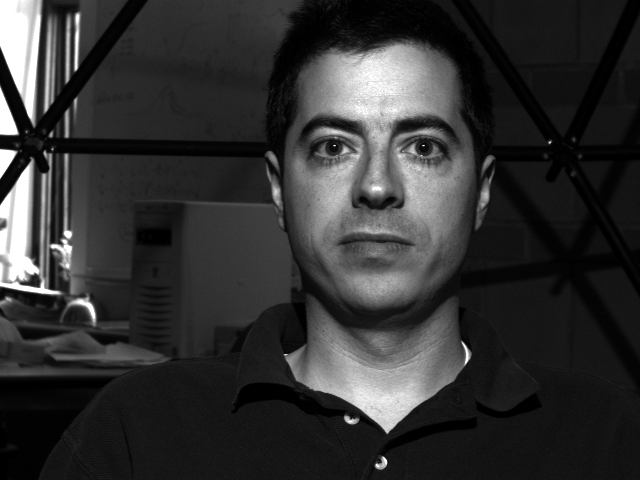
\includegraphics[width=0.22\textwidth]{collection_ps/images/yaleb/yaleB06_P00A+000E+20} \hfill
    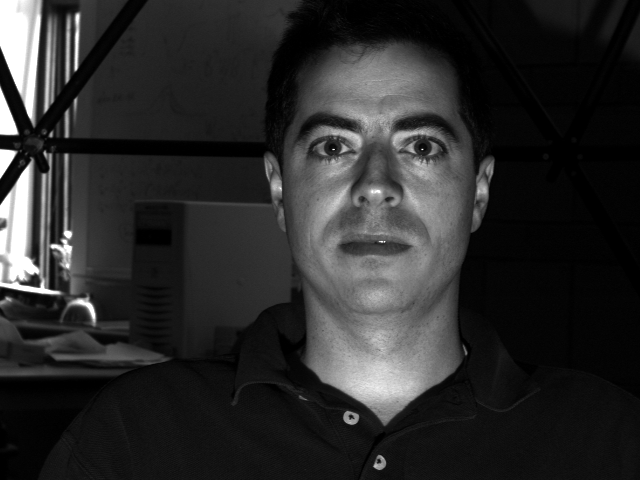
\includegraphics[width=0.22\textwidth]{collection_ps/images/yaleb/yaleB06_P00A+000E-20} \hfill
    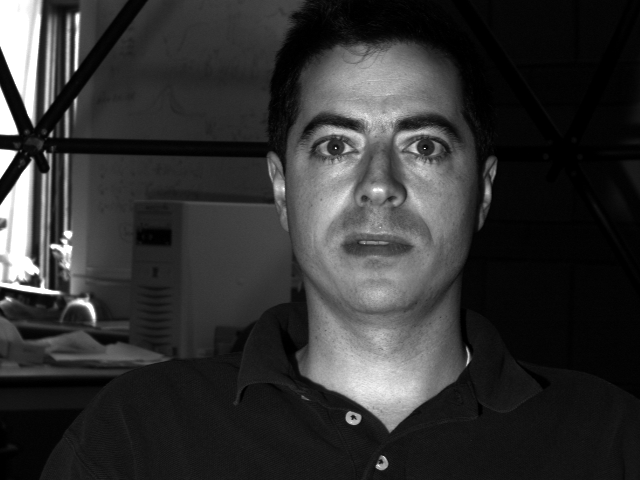
\includegraphics[width=0.22\textwidth]{collection_ps/images/yaleb/yaleB06_P00A+005E-10} \hfill
    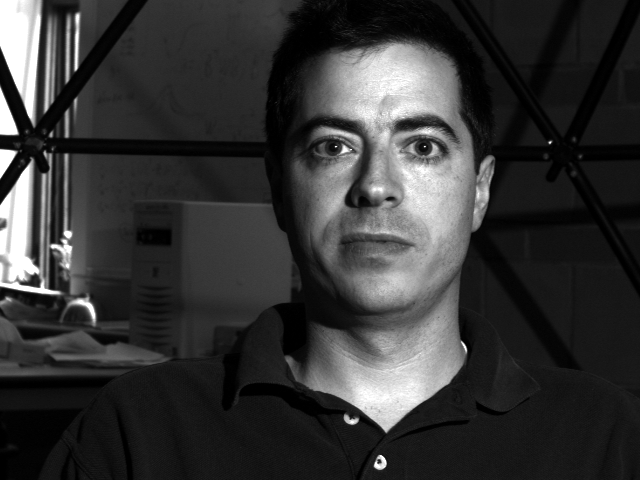
\includegraphics[width=0.22\textwidth]{collection_ps/images/yaleb/yaleB06_P00A-020E+10}
    \hspace*{\fill}
    \caption{An example of unintentional movement during capture of a live
             human subject, from the Yale-B database~\cite{georghiades2001fromfew}.
             This movement violates the pixel-wise correspondence assumption
             made by traditional Calibrated and Uncalibrated Photometric
             Stereo.}
\label{fig:imag_coll_yaleb_movement_example}
\end{figure*}
%%%%%%%%%%%%%%%%%%%%%%%%%%%%%%%%%%%%%%%%

In particular, we recover the shape of the object by exploiting the
similarity within the object \textit{class}.
In the case of faces, there are millions of
available images that can be utilised to build ``in-the-wild'' models. These images
were captured under a large variety of illumination conditions which can be
leveraged in order to recover an estimate of a generic facial shape model.
However, recovering shape from these images is incredibly challenging, as they have been
captured in completely unconstrained conditions. No knowledge of the lighting
conditions, the facial location or the camera geometric properties are provided
with the images. Thus, there are two primary issues that must be solved in
order to perform a class-specific Photometric Stereo decomposition. The first
is that the input images, though of the same object class, are not
pixel-wise aligned. This is a hard requirement for the matrix factorisation
algorithms commonly employed by PS methods. Although challenging, recent
advancements in facial landmark localisation~\cite{cootes2001active} have
provided methods for achieving coarse alignment between facial images within
these ``in-the-wild'' image collections. We employ this approximate alignment
in order to provide a canonical reference space within which to perform
a PS decomposition. Given the aligned ``in-the-wild'' images, we propose to
recover a \textit{class-specific} spherical harmonic (SH)
basis that exploits the low-rank structure of
faces~\cite{georghiades2001fromfew,Basri:2003ie}. Spherical harmonics are ideal for
this purpose as they can be approximated by a low-dimensional linear subspace
\cite{Basri:2003ie,ramamoorthi2001relationship}.
By using the first order SH, up to $90\%$~\cite{yuille1999determining} of
the low-frequency component of the lighting may be approximated for images
of a human face~\cite{Basri:2003ie,%
basri2007photometric,yuille1999determining}. The first order SH
can then be used to recover 3D shape as their discrete approximation directly
incorporates the normals of the object. Given the ``in-the-wild'' nature of
the input images, it is highly likely that some of the images will contain
outliers such as occlusions and artifacts relating to head-pose. A naive
least-squares solution to the decomposition would be heavily biased
by these outliers. Therefore, we propose a decomposition that seeks to
automatically identify these sparse outliers and reduce their effect on
the recovery of the SH basis.
\cref{tbl:imag_coll_different_ps_methods} provides a brief
overview of the difference in assumptions between traditional PS/U-PS and the
proposed class-specific PS.\@
%%%%%%%%%%%%%%%%%%%%%%%%%%%%%%%%%%%%%%%%
\begin{table}
    \centering
    \begin{tabular}{@{}lcccl@{}}
    \toprule
    \textbf{Method}                     & \textbf{\# of Subjects}   & \textbf{Known Lights} & \textbf{Pre-Aligned} & \textbf{Equation}                                      \\ \midrule
    PS                                  & $1$                       & $\cm$                 & $\cm$                & $\bb{X} = \bb{N} \bb{\tilde{L}}$                       \\
    Uncalibrated PS                     & $1$                       & \xmark                & $\cm$                & $\bb{X} = \bb{N} \bb{L}$                               \\
    Class-specific PS                   & $N$                       & \xmark                & \xmark               & $\bb{X} = \bb{B} \bb{P} = \bb{B} (\bb{L} \ast \bb{C})$ \\ \bottomrule
    \end{tabular}
    \caption{A summary of the input requirements for the Photometric Stereo (PS)
             methods considered in this chapter.}
\label{tbl:imag_coll_different_ps_methods}
\end{table}
%%%%%%%%%%%%%%%%%%%%%%%%%%%%%%%%%%%%%%%%

Although a challenging scenario, previous works have considered the recovery
of facial shape from unconstrained image collections.
Typically, this involves
solving some form of Uncalibrated Photometric Stereo problem
\cite{basri2007photometric,papadhimitri2014closed,papadhimitri2014closed,georghiades2001fromfew}.
However, traditional U-PS techniques still assume that images of a single object are
provided by a photometric stereo system under explicit yet unknown directed lighting.
The relaxation of the U-PS problem to a class of
objects further increases the ambiguity inherent within the problem.
Specifically, it is now necessary to separate the illumination variation
from the identity and deformation between the objects.
This problem has been approached for both shape recovery and
facial recognition purposes
\cite{lee2005bilinear,lee2005estimation,minsik2014realtime,minsik2013robust,zhou2007appearance}.
\citet{lee2005bilinear,lee2005estimation} recover facial shape by separating illumination
from identity in a manner that is similar to 3DMMs.
\citet{minsik2014realtime,minsik2013robust} separate the appearance and identity
via a low rank tensor decomposition that provides a very efficient
reconstruction methodology.
However, all of these methods still require an explicit dense 3D model in order
to perform their decomposition.
\citet{georghiades2001fromfew} built a generative model of facial appearance
by exploiting the U-PS problem. However, they focused primarily on using
this model for facial recognition rather than focusing on the quality of the
reconstruction. Their key insight was that multiple images of a single face
under varying illumination forms a convex cone in the space of images that can
be used as a generative model. They proposed to resolve the ambiguities that
arise at depth reconstruction time through facial symmetry. Specifically, they
assumed bilateral symmetry in that the top and bottom of the face must lie at
approximately the same depth for a frontal image.

\citet{KemelmacherShlizerman:2013iv} proposed a method for automatically
building morphable models from unconstrained ``in-the-wild'' images of faces
acquired from the Internet. This is an extension of their previous work
on building person-specific models from Internet photos~\cite{kemelmacher2011face}
which concentrates on creating clusters of individuals that are portraying
the same emotion. Semantic queries such as ``smiling baby'' were used in order
to collect sets of images, called clusters, that contain different individuals
with the same semantic expression (all babies, all smiling).
Within a cluster, the method of
\citet{kemelmacher2012collection} is used to align all of the faces to a
per-cluster average face. Given a number of these clusters, for example
``smiling baby'', ``crying baby'', ``smiling adult'', the per-cluster averages
are aligned to a global average that allows transfer of expression and
semantic meaning between clusters. \citet{KemelmacherShlizerman:2013iv} also
proposes to perform a single-view reconstruction via an ad-hoc decomposition
that seeks to decouple illumination and deformation. Our class-specific
PS extends this decomposition in two ways. Firstly, we
provide the explicit algebraic form of this decomposition and explain its
connection to existing factorisation literature. Secondly, we extend the
factorisation to incorporate a low rank
constraint~\cite{candes2011robust,peng2012rasl,sagonas2014raps,cheng2013rank,%
wu2010robust,lu2013uncalibrated} to help remove sparse outliers
whilst maintaining the low frequency lighting variations. Although this shares a
similar optimisation framework to other
robust principal component analysis problems such as
\cite{candes2011robust,peng2012rasl,wu2010robust,lu2013uncalibrated},
we are the first to propose a low-rank decomposition that recovers a subspace
of spherical harmonics. Furthermore, in contrast to \citet{KemelmacherShlizerman:2013iv}
we attempt to build a single global model of illumination and deformation
that is inspired by global models of appearance and shape such as
Active Appearance Models (AAMs)~\cite{cootes2001active}. By performing a coarser
alignment using modern facial landmark localisation methods, rather than
the time-consuming optical flow performed by \citet{KemelmacherShlizerman:2013iv},
our training time is substantially reduced.
It also allows our recovered basis to be coupled with facial alignment
techniques for simultaneous facial landmark localisation and dense surface
recovery.
\cref{fig:imag_coll_overview} provides an overview of our proposed algorithm
for recovering facial shape from unconstrained image collections.
%%%%%%%%%%%%%%%%%%%%%%%%%%%%%%%%%%%%%%%
\begin{figure}[t]
    \centering
    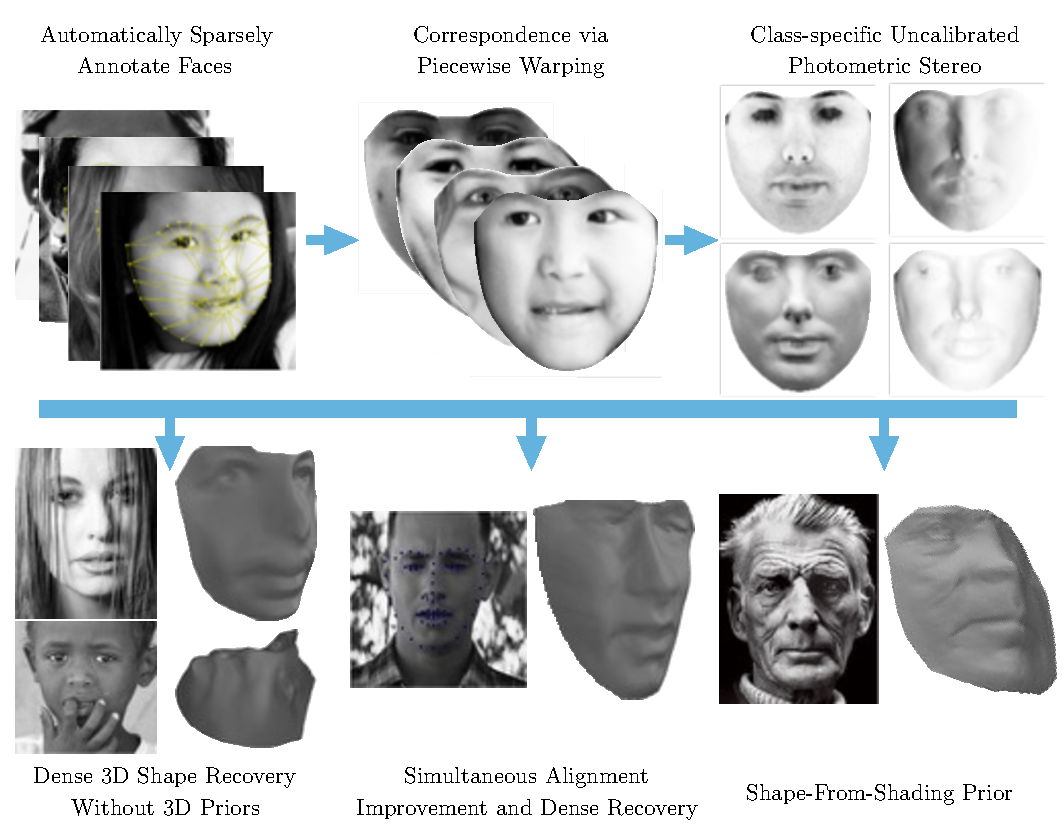
\includegraphics[width=15cm]{collection_ps/images/algorithm_overview}
    \caption{An overview of our proposed approach. Given a set of
             ``in-the-wild'' images, we coarsely align them using an efficient
             facial landmark localisation technique and then perform our
             novel robust class-specific PS.\@ The recovered Spherical Harmonic
             basis has a number of uses that are presented in
             \cref{sec:imag_coll_experiments}.}
\label{fig:imag_coll_overview}
\end{figure}
%%%%%%%%%%%%%%%%%%%%%%%%%%%%%%%%%%%%%%%

The remainder of the chapter will proceed as follows: \cref{sec:imag_coll_problem}
outlines our approach to class-specific PS and explains the explicit matrix
factorisation form of the decomposition proposed by
\citet{KemelmacherShlizerman:2013iv}. We then extend the least-squares
solution of the problem proposed by \citet{KemelmacherShlizerman:2013iv} to
incorporate a low-rank prior that is robust to sparse outliers.
\cref{sec:imag_coll_experiments} provides a comparison of our low-rank
decomposition with our least-squares decomposition~\cite{KemelmacherShlizerman:2013iv}
on an ``in-the-wild'' collection of images. We also investigate the suitability
of the recovered basis as a shape-from-shading prior, as described in
\cref{sec:singl_img_gsfs} and as a person specific appearance model for
AAM~\cite{cootes2001active} fitting. Finally, in \cref{sec:imag_coll_summary},
we provide a summary of the chapter and draw conclusions on our results.
%%%%%%%%%%%%%%%%%%%%%%%%%%%%%%%%%%%%%%%%%%%%%%%%%%%%%%%%%%%%%%%%%%%%%%%%%%%%%%%%
%%%%%%%%%%%%%%%%%%%%%%%%%%%%%%%%%%%%%%%%%%%%%%%%%%%%%%%%%%%%%%%%%%%%%%%%%%%%%%%%
\section{Problem Formulation}\label{sec:problem}
%%%%%%%%%%%%%%%%%%%%%%%%%%%%%%%%%%%%%%%%%%%%%%%%%%%%%%%%%%%%%%%%%%%%%%%%%%%%%%%%
In this section we describe how a spherical harmonic (SH) basis can be recovered
using uncalibrated photometric stereo (PS) techniques. We then describe how this
problem generalises to a multi-person dataset and how a representation of shape
can be recovered per image. Finally, we discuss the importance of achieving
correspondence between the images in an efficient and scalable manner.
%%%%%%%%%%%%%%%%%%%%%%%%%%%%%%%%%%%%%%%%%%%%%%%%%%%%%%%%%%%%%%%%%%%%%%%%%%%%%%%%
\subsection{Spherical Harmonic Bases}\label{subsec:spherical_harmonic}
%%%%%%%%%%%%%%%%%%%%%%%%%%%%%%%%%%%%%%%%%%%%%%%%%%%%%%%%%%%%%%%%%%%%%%%%%%%%%%%%
The lambertian reflectance model states that matte materials reflect light
uniformly in all directions. This simple image formation model assumes that the
intensity of light reflecting from a surface is a function of the shape of the
surface and a linear combination of point light sources. More formally, given an
image $I(x, y)$, the intensity at a given pixel $(x, y)$ of a convex lambertian
surface illuminated by a single light, can be expressed as
%%%%%%%%%%%%%%%%%%%
\begin{equation}\label{eq:lambert_law}
    I(x, y) = \rho(x, y) \bb{l}^T \bb{n}(x, y),
\end{equation}
%%%%%%%%%%%%%%%%%%%
where $\rho(x, y)$ is the albedo at the pixel and represents surface
reflectivity, $\bb{l}$ is the vector denoting the single point light source
illuminating the object and $\bb{n}(x, y)$ is the surface normal at the
pixel.

If we now consider a collection of directional light sources placed at infinity,
the lighting intensity at a given pixel can be expressed as a non-negative
function of the unit sphere using a sum of spherical harmonics. Formally,
%%%%%%%%%%%%%%%%%%%
\begin{equation}\label{eq:spherical_harmonics}
    I(x, y) = \sum^{\infty}_{n=0} \sum^{n}_{m=-n} \alpha_n \; \ell_{nm} \; \rho(x,y) \; Y_{nm}(\bb{n}(x,y)),
\end{equation}
%%%%%%%%%%%%%%%%%%%
where $\alpha_n = \pi, 2\pi/3, \pi/4, \ldots$, $\ell_{nm}$ are the coefficients
of the harmonic expansion of the lighting and $Y_{nm}(\bb{n}(x,y))$ are the
surface SH functions evaluated at the surface normal, $\bb{n}(x,y)$. As
$n \rightarrow \infty$, the coefficients tend to zero, and thus the SH can be
accurately represented by the lower order harmonics. \citet{RefWorks:316}, it
was shown that the first order SH function is guaranteed to represent at least
$87.5\%$ of the reflectance and experimentally verified to recover up to $95\%$
in the case of faces. The first order SH expansion is also directly related to
the objects surface normals:
%%%%%%%%%%%%%%%%%%%
\begin{equation}\label{eq:first_order_spherical_harmonics}
    \begin{aligned}
        \bb{Y}(\bb{n}(x, y))  = \rho(x, y) {[ 1, \bb{n}_{x}(x, y), \bb{n}_{y}(x, y), \bb{n}_{z}(x, y) ]}^T,
   \end{aligned}
\end{equation}
%%%%%%%%%%%%%%%%%%%
where $\bb{n}_{i}(x, y)$ denotes the $i$th component of the normal vector. 
This is a particularly useful result as recovering the first order SH means 
directly recovering a representation of shape for an object.
%%%%%%%%%%%%%%%%%%%%%%%%%%%%%%%%%%%%%%%%%%%%%%%%%%%%%%%%%%%%%%%%%%%%%%%%%%%%%%%%
\subsection{Uncalibrated Photometric Stereo}\label{subsec:uncalibrated_ps}
%%%%%%%%%%%%%%%%%%%%%%%%%%%%%%%%%%%%%%%%%%%%%%%%%%%%%%%%%%%%%%%%%%%%%%%%%%%%%%%%
Classical photometric stereo (PS) seeks to recover the normals of a convex
object given a number of images under known different lighting with known
directions. Traditionally, the following decomposition is performed
%%%%%%%%%%%%%%%%%%%
\begin{equation}\label{eq:general_ps}
    \bb{X} = \bb{N} \tilde{\bb{L}},
\end{equation}
%%%%%%%%%%%%%%%%%%%
where $\bb{X} \in \bb{R}^{d \times n}$ is the matrix of observations,
and each of the $n$ columns represents a vectorised image of the object with $d$
total pixels, $\bb{N} \in \bb{R}^{d \times 3}$ contains the normal at
every pixel and $\tilde{\bb{L}} \in \bb{R}^{3 \times n}$ is the matrix
of lighting vectors per image. Assuming accurate light vectors and no shadowing
artifacts, this problem is trivially solved as a linear least squares problem.
Photometric stereo has been shown to provide accurate facial reconstructions
despite faces not representing true lambertian objects. For example, there are
many publicly available facial PS datasets such as the 
Photoface Database~\cite{RefWorks:293} and the 
Yale B~\cite{Georghiades:2001ft} dataset.

If the lighting vectors are inaccurate or unknown, then PS is said to be
uncalibrated. \citet{Basri:2006fo} showed that $\bb{X}$ can
be decomposed via a rank constrained singular value decomposition (SVD) to
recover the SH bases and the lighting coefficients in the uncalibrated setting.
First order SH are recovered by a rank 4 SVD and are accurate up to a $4 \times 4$ 
generalised Lorentz transformation. By enforcing constraints such as the
integrability constraint~\cite{RefWorks:99}, the first order SH, and thus the
normals, can be recovered up to a generalised bas relief ambiguity (GBR).
Formally, uncalibrated PS looks to recover
%%%%%%%%%%%%%%%%%%%
\begin{equation}\label{eq:uncalibrated_ps}
    \bb{X} = \bb{B} \bb{L},
\end{equation}
%%%%%%%%%%%%%%%%%%%
where $\bb{X}$ is as before, $\bb{B} \in \bb{R}^{d \times 4}$ 
contains the first order SH basis images and
$\bb{L} \in \bb{R}^{4 \times n}$ is the matrix of lighting coefficients. 
As previously mentioned, the solution to this problem is found by performing an
SVD,
$\bb{X} =\nobreak \bb{U} \bb{\Sigma} \bb{V}^T$, $\bb{B} = \bb{U} \sqrt{\bb{\Sigma}}$
and $\bb{L} = \sqrt{\bb{\Sigma}} \bb{V}^T$. 
Uncalibrated PS is useful as it is not always possible to recover accurate 
lighting estimations for every image.
%%%%%%%%%%%%%%%%%%%%%%%%%%%%%%%%%%%%%%%%%%%%%%%%%%%%%%%%%%%%%%%%%%%%%%%%%%%%%%%%
\subsection{Class Specific Uncalibrated Photometric Stereo}\label{subsec:class_uncalibrated_ps}
%%%%%%%%%%%%%%%%%%%%%%%%%%%%%%%%%%%%%%%%%%%%%%%%%%%%%%%%%%%%%%%%%%%%%%%%%%%%%%%%
A generalisation of the uncalibrated PS problem for a specific class involves
recovering a joint basis of appearance and illumination. In the case of SH for
faces, this means attempting to separate the identity of the individual from
their surface normals. This problem is a classic example of a bilinear
decomposition problem and has been previously studied for use in 3D surface
recovery~\cite{Zhou:bl,RefWorks:306,RefWorks:307,Lee:2005bc,RefWorks:311}. In
the case of SH, we seek to recover a low dimensional linear subspace that can
recover normals for multiple individuals. This subspace implies that a face can
be accurately reconstructed using a linear combination of basis shapes. This
assumption is commonly employed in algorithms such as the 3DMM and AAMs.
Assuming that we want to recover $k$ such components for our shape subspace, and
that we are using the first order SH, we will recover a $d \times 4k$ basis
matrix that allows us to recover 3D facial shape for multiple individuals.
Formally,
%%%%%%%%%%%%%%%%%%%%%%%%%%
\begin{equation}\label{eq:class_specific_ps}
        \bb{X} = \bb{B} (\bb{L} \ast \bb{C}),
\end{equation}
%%%%%%%%%%%%%%%%%%%%%%%%%%
where $\bb{B} \in \bb{R}^{d \times 4k}$ is the linear basis,
$\bb{L} \in \bb{R}^{4 \times n}$ is the matrix of first order SH lighting
coefficients, $\bb{C} \in \bb{R}^{k \times n}$ is the matrix of shape
coefficients and $(\cdot \ast \cdot)$ denotes the Khatri-Rao
product~\cite{Khatri:1968dj}. In fact, this is the exact decomposition problem
solved by \citet{RefWorks:311} where they denote the combined coefficients
matrix as $\bb{P} = \bb{L} \ast \bb{C}$. This was partially
recognised by \citet{Zhou:bl}, however they recover the lighting and shape
coefficient separately by iteratively solving for each in an alternating
fashion. \citet{Zhou:bl} also do not provide any examples of the quality of the
shape estimate that they recover.

\citet{RefWorks:306,RefWorks:307} also attempt this decomposition by
posing the problem in the form of a tensor. The decomposition can then be solved
by applying a multilinear SVD.\@ However, multilinear SVD requires a tensor
representation and thus these techniques require prior data to recover results.
A tensor representation is useful, however, for illustrating how to recover the
$d \times 4$ first order SH for an individual, given their coefficients vector
$\bb{c}_i \in \bb{R}^{k \times 1}$. We reshape the basis matrix
$\bb{B}$ as a tensor which we denote $\bb{S} \in \bb{R}^{d \times k
\times 4}$. The tensor product along the second mode, $\bb{S} \times_2 \bb{c}_i$, 
recovers the person specific shape of the $i$th column of
$\bb{X}$. To recover $\bb{B}$ from $\bb{S}$, we perform
matricisation of $\bb{S}$ along the first mode, denoted $\bb{S}_{(1)}$,
to yield $\bb{S}_{(1)} = \bb{B} \in \bb{R}^{d \times 4k}$.

The problem given in~\eqref{eq:class_specific_ps} can now be solved within an
optimisation framework, which we examine in detail in the next section.
%%%%%%%%%%%%%%%%%%%%%%%%%%%%%%%%%%%%%%%%%%%%%%%%%%%%%%%%%%%%%%%%%%%%%%%%%%%%%%%%
\subsection{Robust Construction Of Spherical Harmonic Bases}\label{subsec:robust_sh_basis}
%%%%%%%%%%%%%%%%%%%%%%%%%%%%%%%%%%%%%%%%%%%%%%%%%%%%%%%%%%%%%%%%%%%%%%%%%%%%%%%%
Inspired by recent advances in robust low-rank subspace
recovery~\cite{RefWorks:321}, we seek to modify \cref{eq:class_specific_ps} to
include new constraints that impose robustness. As mentioned previously, faces
can be accurately reconstructed by a linear combination of faces taken from a
low-dimensional basis. Therefore, we propose to decompose the image matrix into
a low-rank part ($\bb{A}$) capturing the low frequency shape information and a
sparse part ($\bb{E}$) accounting for gross but sparse noise such as partial
occlusions and pixel corruptions. To promote low-rank and sparsity the nuclear
norm (denote by $\lVert \bb{\cdot} \rVert_{*}$) and the $\ell_1$-norm (denote by
$\lVert \bb{\cdot} \rVert_{1}$) are employed, respectively. Formally we propose
to solve the following non-convex optimisation problem:
%%%%%%%%%%%%%%%%%%%
\begin{equation}
\begin{aligned}
    &\argmin_{\bb{A},\bb{E},\bb{B},\bb{L},\bb{C}} & &\lVert \bb{A} \rVert_{*} + \lambda \lVert \bb{E} \rVert_{1} + \frac{\mu}{2} \lVert \bb{A} - \bb{B} (\bb{L} \ast \bb{C}) \rVert^{2}_{F} \\
    & \text{subject to} & & \bb{X} = \bb{A} + \bb{E}, \; \bb{B}^T \bb{B} = \bb{I}.
\end{aligned}
\label{eq:robust_sh_problem}
\end{equation}
%%%%%%%%%%%%%%%%%%%
Although the above problem is non-convex, an accurate solution can be obtained
by employing the Alternating Directions Method (ADM)~\cite{Bertsekas1982}. That
is, to minimise the following augmented Lagrangian function:
%%%%%%%%%%%%%%%%%%%
\begin{equation}
    \begin{aligned}
        \mathcal{L}(\bb{A},\bb{E},\bb{B},\bb{C},\bb{L},\bb{Y}) &= \lVert \bb{A} \rVert_{*} + \lambda \lVert \bb{E} \rVert_{1} + \frac{\mu}{2} \lVert \bb{A} - \bb{B} (\bb{L} \ast \bb{C}) \rVert^{2}_{F} \quad + \\
        & \quad \Tr{(\bb{Y}^T(\bb{X} - \bb{A} - \bb{E}))} +  \frac{\mu}{2} \lVert \bb{X} - \bb{A} - \bb{E} \rVert_{F}^{2},
    \end{aligned}\label{eq:augmented_lagrangian}
\end{equation}
%%%%%%%%%%%%%%%%%%%
with respect to $\bb{B}^T \bb{B} = \bb{I}$. Let $t$ denote the iteration index. 
Given $\bb{A}_{[t]}$, $\bb{E}_{[t]}$, $\bb{B}_{[t]}$, $\bb{C}_{[t]}$, $\bb{L}_{[t]}$, $\bb{Y}_{[t]}$
and $\mu_{[t]}$, the iteration of ADM for \cref{eq:robust_sh_problem} reads:
%%%%%%%%%%%%%%%%%%%
\begin{align}
    \bb{A}_{[t+1]} &= \lVert \bb{A}_{[t]} \rVert_{*} + \frac{\mu_{[t]}}{2} \biggl( \lVert \bb{A}_{[t]} - \bb{B}_{[t]} (\bb{L}_{[t]} \ast \bb{C}_{[t]}) \rVert^{2}_{F} + \lVert \bb{X} - \bb{A}_{[t]} - \bb{E}_{[t]} + \frac{\bb{Y}_{[t]}}{\mu_{[t]}} \rVert_{F}^{2} \biggr), \label{eq:text_A_update} \\
    \bb{B}_{[t+1]} &= \argmin_{\bb{B}_{[t]}^T \bb{B}_{[t]} = \bb{I}} \frac{\mu_{[t]}}{2} \lVert \bb{A}_{[t+1]} - \bb{B}_{[t]} (\bb{L}_{[t]} \ast \bb{C}_{[t]}) \rVert_{F}^{2}, \label{eq:text_B_update} \\
    \left[ \bb{L}_{[t+1]}, \bb{C}_{[t+1]} \right] &= \argmin_{\bb{L}_{[t]}, \bb{C}_{[t]}} \frac{\mu_{[t]}}{2} \lVert \bb{A}_{[t+1]} - \bb{B}_{[t+1]} (\bb{L}_{[t]} \ast \bb{C}_{[t]}) \rVert_{F}^{2}. \label{eq:text_LC_update}
\end{align}
%%%%%%%%%%%%%%%%%%%
Subproblem~\eqref{eq:text_A_update} admits a closed-form solution, given by the
singular value thresholding (SVT)~\cite{Cai:2010hz} operator as:
%%%%%%%%%%%%%%%%%%%
\begin{equation}\label{eq:text_A_SVT}
    \bb{A}_{[t+1]} = D_{\mu_{[t]}^{-1}} \left[ \bb{M}_{[t]}  - \bb{A}_{[t]} + \bb{X} - \bb{E}_{[t]} + \frac{\bb{Y}_{[t]}}{\mu_{[t]}} \right],
\end{equation}
%%%%%%%%%%%%%%%%%%%
where $\bb{M}_{[t]} = \bb{B}_{[t]} (\bb{L}_{[t]} \ast \bb{C}_{[t]})$ is introduced 
for brevity of the equation and the SVT is defined as
$D_{\tau}(\bb{Q}) = \bb{U} \bb{S}_{\tau} \bb{V}^T$ for any matrix $\bb{Q}$ with SVD:\@
$\bb{Q} = \bb{U} \bb{S} \bb{V}^T$. 
Subproblem~\eqref{eq:text_E_update} has a unique solution that is obtained via 
the elementwise shrinkage operator~\cite{RefWorks:321}. The shrinkage operator 
is defined as $\mathcal{S}_{\tau}[q]=\mbox{sgn}(q) \: \max(|q|-\tau, 0)$. 
Therefore, the solution of~\eqref{eq:text_E_update} is
%%%%%%%%%%%%%%%%%%%
\begin{equation}\label{eq:text_E_shrinkage}
    \bb{E}_{[t+1]} = \mathcal{S}_{\lambda \mu_{[t]}^{-1}} \left[ \bb{X} - \bb{A}_{[t+1]} + \frac{\bb{Y}_{[t]}}{\mu_{[t]}} \right].
\end{equation}
%%%%%%%%%%%%%%%%%%%
{ % Courtesy of the wonderful Georgios!
%%%%%%%%%%%%%%%%%%%
\def\t#1{{\bb{#1}_{[t]}}}
\def\tp#1{{\bb{#1}_{[t+1]}}}
%%%%%%%%%%%%%%%%%%%
\noindent Subproblem~\eqref{eq:text_B_update} is a reduced rank Procrustes
Rotation problem~\cite{RefWorks:327}. Its solution is given by
$\bb{B}_{[t]} = \bb{U} \bb{V}^{\top}$ with
%%%%%%%%%%%%%%%%%%%
\begin{equation}\label{eq:text_B_update2}
    \tp A {\left(\t L \ast \t C\right)}^{\top} = \bb{U} \bb{\Sigma} \bb{V^{\top}},
\end{equation} 
%%%%%%%%%%%%%%%%%%%
being the SVD of $\tp A {\left(\t L \ast \t C\right)}^{\top}$. However, due the
unitary invariance of the Frobenius norm, Equation~\ref{eq:text_LC_update}
becomes
%%%%%%%%%%%%%%%%%%%
\begin{equation}\label{eq:text_LC_update2}
    \argmin_{\bb{L}_{[t+1]}, \bb{C}_{[t+1]}} \lVert \bb{B}_{[t+1]}^T\bb{A}_{[t+1]} - \bb{L}_{[t]} \ast \bb{C}_{[t]} \rVert_{F}^{2}.
\end{equation}
%%%%%%%%%%%%%%%%%%%
Subproblem~(\ref{eq:text_LC_update},~\ref{eq:text_LC_update2}) is a least 
squares factorisation of a Khatri-Rao product~\cite{Roemer:2010iv}, which is 
solved as follows:
Let $\bb{Q} = \tp B^{\top} \tp A, \bb{L} = \t L, \text{and} \; \bb{C} = \t C$. 
Furthermore, let $\bb{q}_i, \bb{l}_i, \text{and} \; \bb{c}_i$ be the $i_{th}$ 
columns of 
matrices $\bb{Q}, \bb{L}, \text{and} \; \bb{C}$, respectively. 
Clearly $\bb{q}_i = \bb{l}_i \oplus \bb{c}_i$, where $\oplus$ denotes the Kronecker 
product. For each column of $\bb{Q}$: Reshape $\bb{q}_i$ into a 
matrix $\tilde{\bb{Q}}_i \in \bb{R}^{4 \times k}$ 
such that 
$\text{vec}\left(\tilde{\bb{Q}}_i\right) = \bb{q}_i$. 
Obviously, $\tilde{\bb{Q}}_i = \bb{c}_i \cdot {\bb{l}_i}^{\top}$ is a rank-one matrix.
Compute the SVD of
$\tilde{\bb{Q}}_i$ as $\tilde{\bb{Q}}_i = \bb{U}_i \bb{\Sigma}_i {\bb{V}_i}^{\top}$. 
The best rank-one approximation of $\tilde{\bb{Q}}_i$ is obtained by truncating the SVD as:
$\bb{l}_i = \bb{u}_i \sqrt{\sigma_1}$ and $\bb{c}_i = \sqrt{\sigma_1} \bb{v}_i$,
where $\bb{u}_i$ and $\bb{v}_i$ are the first column vectors of $\bb{U}_i$
and $\bb{V}_i$, respectively, and $\sigma_1$ is the largest singular value.
The ADM for solving~\eqref{eq:robust_sh_problem} is outlined in 
\cref{alg:adm_solution}.
}

It is important to note that there are inherent ambiguities in this
decomposition, both from the SVD to recover $\bb{B}$ and in the Khatri-Rao
factorisation to recover $\bb{L}$ and $\bb{C}$. In particular, we are most
concerned about how they may affect the recovered normals before we integrate
them to recover depth. In order to resolve these ambiguities, we take the
simplest possible approach, we recover the ambiguity matrix from a template set
of normals provided by a known mean face.
%%%%%%%%%%%%%%%%%%%%%%%%%%%%%%%%%%%%%%%%%%%%%%%%%%%%%%%%%%%%%%%%%%%%%%%%%%%%%%%%
%%%%%%%%%%%%%%%%%%%%%%%%%%%%%%%%%%%%%%%%%%%%%%%%%%%%%%%%%%%%%%%%%%%%%%%%%%%%%%%%
\begin{algorithm}[t]
    \caption{Solving~\eqref{eq:robust_sh_problem} by the ADM method.}
\label{alg:adm_solution}
    {\scriptsize\textbf{Input:} Data Matrix $\bb{X} \in \mathbb{R}^{d \times n}$ and parameter $\lambda$.} \\
    {\scriptsize\textbf{Output:} Matrices $\bb{A}$, $\bb{E}$, $\bb{B}$, $\bb{C}$, $\bb{L}$.}  \\
{
    \scriptsize
    % Define commands
    \def\At{{\bb{A}_{[t]}}}
    \def\Et{{\bb{E}_{[t]}}}
    \def\Ct{{\bb{C}_{[t]}}}
    \def\Lt{{\bb{L}_{[t]}}}
    \def\Bt{{\bb{B}_{[t]}}}
    \def\Yt{{\bb{Y}_{[t]}}}
    \def\mut{{\mu_{[t]}}}
    \def\X{{\bb{X}}}
    
    \begin{algorithmic}
        \State{}Initialise: $\bb{A}_{[0]} = 0$, $\bb{E}_{[0]} = 0$, $\bb{B}_{[0]} = 0$, $\bb{C}_{[0]} = 0$, $\bb{L}_{[0]} = 0$, $\bb{Y}_{[0]} = 0$, $\mu_{[0]} = 10^{-6}$, $\rho = 1.1$, $\epsilon = 10^{-8}$
        \While{not converged} %(Outer loop)
            \State{}Fix $\Et$, $\Bt$, $\Ct$, $\Lt$ and update $\bb{A}_{[t + 1]}$ by
                \begin{equation}\label{eq:A_update}
                    \bb{A}_{[t+1]} = D_{\mu_{[t]}^{-1}} \left[  \Bt ( \Lt \ast \Ct ) - \At + \X - \Et + \frac{\Yt}{\mut} \right]
                \end{equation}
            \State{}Fix $\bb{A}_{[t+1]}$, $\Lt$, $\Ct$, $\Lt$ and update $\bb{A}_{[t + 1]}$ by
                \begin{equation}\label{eq:E_update}
                    \bb{E}_{[t+1]} = \mathcal{S}_{\lambda \mut^{-1}} \left[ \X - \bb{A}_{[t+1]} + \frac{\Yt}{\mut} \right]
                \end{equation}
            \State{}Update $\bb{B}_{[t+1]}$ by first performing the SVD on:
                \begin{equation}\label{eq:ALC_svd}
                    \bb{A}_{[t+1]} {(\Lt \ast \Ct)}^T = \bb{U} \bb{\Sigma} \bb{V}, \; \bb{B}_{[t+1]} = \bb{U} \bb{V}^T
                \end{equation}
            \State{}Update $[\bb{L}_{[t+1]}, \bb{C}_{[t+1]}]$ via a Least Squares Khatri-Rao factorization, as described in \cref{subsec:robust_sh_basis}
            \State{} Update Lagrange multipliers by
                \begin{equation}\label{eq:Y_update}
                    \bb{Y}_{[t+1]} = \Yt + \mut \left( \X - \bb{A}_{[t+1]} - \bb{E}_{[t+1]} \right)
                \end{equation}
            \State{}Update $\mu_{[t+1]}$ by $\mu_{[t+1]} = \min(\rho \mut, 10^6)$
            \State{}Check convergence condition
                \begin{equation}\label{eq:convergence_condition}
                    \begin{aligned}
                        &\lVert \X - \bb{A}_{[t+1]} - \bb{E}_{[t+1]} \rVert_{\infty} < \epsilon, \\
                        &\lVert \bb{A}_{[t+1]} - \bb{B}_{[t+1]} - (\bb{L}_{[t+1]} \ast \bb{C}_{[t+1]}) \rVert_{\infty} < \epsilon
                    \end{aligned}
                \end{equation}
            \State{}$t \leftarrow t + 1$
        \EndWhile{}
    \end{algorithmic}
}
\end{algorithm}
%%%%%%%%%%%%%%%%%%%%%%%%%%%%%%%%%%%%%%%%%%%%%%%%%%%%%%%%%%%%%%%%%%%%%%%%%%%%%%%%
%%%%%%%%%%%%%%%%%%%%%%%%%%%%%%%%%%%%%%%%%%%%%%%%%%%%%%%%%%%%%%%%%%%%%%%%%%%%%%%%
%%%%%%%%%%%%%%%%%%%%%%%%%%%%%%%%%%%%%%%%%%%%%%%%%%%%%%%%%%%%%%%%%%%%%%%%%%%%%%%%
\subsection{Efficient Pixelwise Correspondence}\label{subsec:correspondence}
%%%%%%%%%%%%%%%%%%%%%%%%%%%%%%%%%%%%%%%%%%%%%%%%%%%%%%%%%%%%%%%%%%%%%%%%%%%%%%%%
In contrast to the related work of \citet{RefWorks:311},
we achieved pixelwise correspondence between our images by using existing,
efficient sparse facial alignment algorithms. This has two distinct advantages.
Firstly, recent facial alignment algorithms such as those by
\citet{Ren:it} and \citet{Kazemi:he} can produce a very accurate set
of sparse facial features in the order of a single millisecond. In contrast, the
optical flow method cited in \citet{RefWorks:311} takes multiple seconds even for
a small image. This means that our training time is drastically reduced in
comparison to \citet{RefWorks:311}. Ideally, our technique would be able to scale
to the magnitude of thousands of images, whereas the alignment of
\citet{RefWorks:311} would quickly become infeasible as the number of images
increases. In fact, the optical flow step is run multiple times as the
collection flow algorithm is used~\cite{RefWorks:290} which involves an
iterative algorithm of rank 4 decompositions and repeated optical flow.
Secondly, the use of a direct alignment to a single reference frame enables the
the usage of our basis in existing appearance based facial alignment algorithms
such as AAMs. This means that our basis can be used to reconstruct dense 3D
shape of faces directly from an existing AAM fitting provided the reference
space of the AAM and our subspace is the same.

However, it is important to note that there are two potential drawbacks to our
alignment technique. The alignment is based on a Piecewise Affine warping and is
thus much coarser than the optical flow technique used in \citet{RefWorks:311}.
This is particularly amplified when larger poses are present in the input
images. However, this is partly why the low rank component of our algorithm is
so important. As \cref{fig:low_rank_warping} shows, the robust
decomposition of the basis helps correct these large global errors so that the
shape subspace can be successfully recovered. Secondly, our technique does not
contain a number of sub-clusters that can be used to warp expression onto our
model. However, by using a large number of images that contain expression we
directly include expression within our subspace. In \citet{RefWorks:311}, the
recovered subspace will necessarily be devoid of expression as the global
reference shape is neutral. This means that the subspace recovered by
\citet{RefWorks:311} will not be able to recover expressive 3D shape using
efficient facial alignment algorithms.
%%%%%%%%%%%%%%%%%%%%%%%%%%%%%%%%%%%%%%%
% \begin{figure}
%     \centering
%     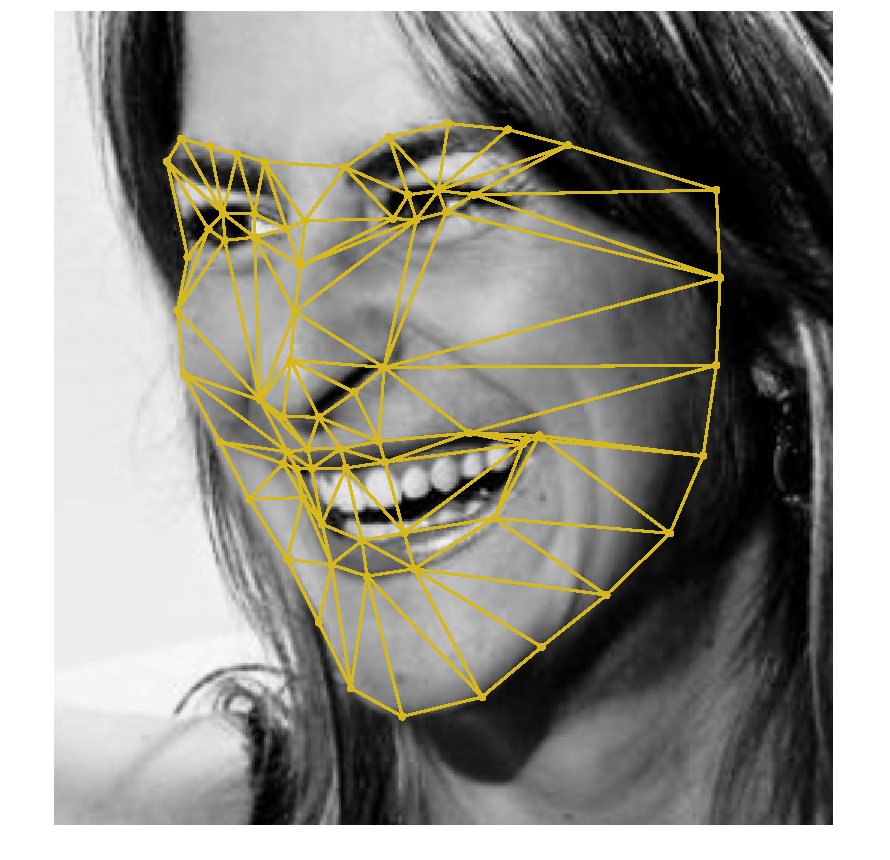
\includegraphics[width=2cm,height=2cm]{images/example_warped_original}
%     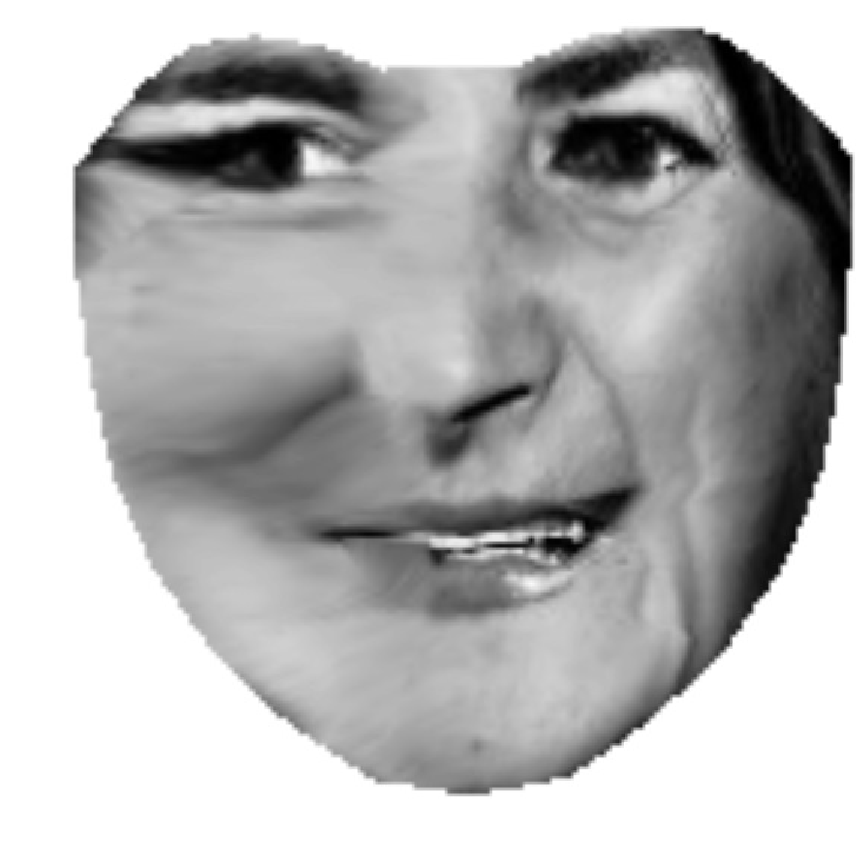
\includegraphics[width=2cm,height=2cm]{images/example_warped}
%     
\includegraphics[width=2cm,height=2cm]{images/example_warped_low_rank}
%     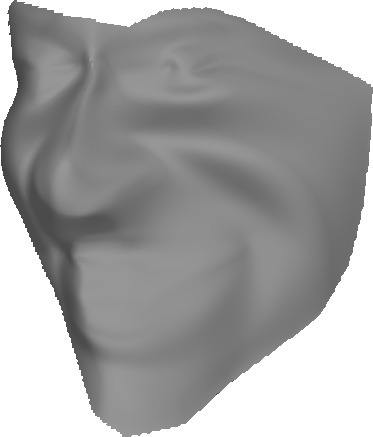
\includegraphics[width=1.8cm,height=1.8cm,trim = 0cm -1cm 0cm 0cm]{images/example_warped_shape}
%     \caption{{\bf Example of the low rank effect on warped pose}. From left to
%              right:
%              initial input image, input image after warping,
%              warped image after the low rank constraint, 
%              recovered depth from warped image.}
% \label{fig:low_rank_warping}
% \end{figure}
%%%%%%%%%%%%%%%%%%%%%%%%%%%%%%%%%%%%%%%
%%%%%%%%%%%%%%%%%%%%%%%%%%%%%%%%%%%%%%%%%%%%%%%%%%%%%%%%%%%%%%%%%%%%%%%%%%%%%%%%
\section{Experiments}\label{sec:imag_coll_experiments}
%%%%%%%%%%%%%%%%%%%%%%%%%%%%%%%%%%%%%%%%%%%%%%%%%%%%%%%%%%%%%%%%%%%%%%%%%%%%%%%%
%%%%%%%%%%%%%%%%%%%%%%%%%%%%%%%%%%%%%%%
\begin{table}
    \centering
    \begin{tabular}{lccccc}
        \toprule
        \textbf{Data}          & \textbf{Warp (s)} & \textbf{Decomposition (s)} & \textbf{Inverse Warp (s)} & \textbf{Total (s)} \\ \midrule
        HELEN (2330 images)    & 8                 & 730                        & 25                        & 763                \\
        Tom Hanks (274 images) & 1                 & 21                         & 4                         & 26                 \\  \bottomrule
    \end{tabular}
    \caption{\textbf{Training Times.} Mean training times in seconds over 10
             runs rounded to the nearest second. ``Warp'' denotes warping to the
             LFPW reference frame of $(150 \times 150)$ pixels, ``Inverse Warp''
             denotes warping back to the original images and ``Decomposition''
             denotes the total training time of our method described in
             \cref{subsec:imag_coll_robust_sh_basis}. Original images were larger than 
             the reference, hence the increase from ``Warp'' to ``Inverse Warp''.
             Timings were recorded on an Intel Xeon E5--1650 3.20GHz with
             32GB of RAM.}
\label{tbl:imag_coll_timings}
\end{table}
%%%%%%%%%%%%%%%%%%%%%%%%%%%%%%%%%%%%%%%
In this section we provide a number of experiments that emphasise the increased
robustness of our reconstructions. We also show a new application to this type
of model that involves improving the fitting results of an AAM using our
constructed SH basis. Choosing the number of components, $k$, to recover is an
important problem that was not properly addressed by Kemelmacher-Schlizerman in
\cite{KemelmacherShlizerman:2013iv}. In these experiments we attempt to recover as many
components as possible in order to strike a balance between cleanly
reconstructed normals and identity. However, there is a trade-off when choosing
the value of $k$. In particular, if the value of $k$ is too large, then the
decomposition is unable to separate the identity and shape and the subspace of
shape no longer represents valid normals. This is one of the primary advantages
of our robust decomposition, as it allows the value of $k$ to be larger given
the reduced rank of the images. However, a potential disadvantage of our
proposed method is the sensitivity of the algorithm to the parameter $\lambda$,
which must be tuned for every dataset. It is also important to stress that our
main goal is to recover the low frequency shape information to provide plausible
3D facial surfaces under challenging conditions. However, in
\cref{subsec:experiments_smith}, we show that our recovered subspace can
be used in existing high frequency recovery algorithms such as SFS.\@

The area of 3D facial surface recovery is lacking any form of formal
quantitative benchmark. The quantitative benchmark presented in
\cite{KemelmacherShlizerman:2013iv} is performed on depth data recovered from photometric
stereo. This is not ground truth depth data, as error is introduced during
integration, and a more accurate evaluation would be the angular error of the
recovered normals. However, in the presence of cast shadows, even the normals of
photometric stereo are biased. For this reason, the lack of a standard and fair
quantitative evaluation, we focus on qualitative results in this paper.

Specifically we performed the following experiments: (1) We built our subspace
using the HELEN~\cite{le2012interactive} dataset. We directly compare against the
blind decomposition proposed in~\cite{KemelmacherShlizerman:2013iv} and show particularly
challenging images from the dataset. This experiment highlights the difficulty
in constructing subspaces from large a set of in-the-wild images. (2) We show
that the robust subspace learnt in (1) can be used within the shape-from-shading
(SFS) framework of \citet{smith2006recovering}. By recovering the normals
from every image of HELEN, we can perform a secondary principal component
analysis (PCA) on the normals in order to directly embed them within Smith's
algorithm. In this experiment, we compare against a clean dataset of normals
acquired from the ICT-3DRFE~\cite{stratou2012exploring} database. (3) We show how our
subspace can be combined with an existing facial alignment algorithm, namely
project-out AAMs~\cite{matthews2004active}. Our subspace can be used both as the
appearance basis for the AAM and also as a methodology of recovering dense 3D
shape.

In the following section we describe the construction of the bases and explain
what processing was performed on each dataset.
%%%%%%%%%%%%%%%%%%%%%%%%%%%%%%%%%%%%%%%%%%%%%%%%%%%%%%%%%%%%%%%%%%%%%%%%%%%%%%%%
\subsection{Constructing The Robust Bases}\label{subsec:construction}
%%%%%%%%%%%%%%%%%%%%%%%%%%%%%%%%%%%%%%%%%%%%%%%%%%%%%%%%%%%%%%%%%%%%%%%%%%%%%%%%
The process of building the robust SH basis was the same for all datasets
involved. Facial annotations consisting of 68 points were recovered through
various methods for each dataset. In the case of the HELEN database, the manual
annotations provided by the IBUG group were used~\cite{sagonas2013300,sagonas2013semi},
in the case of the Yale B, Photoface and ICT-3DRFE databases, manual annotations
were used and the in-the-wild images and video of Tom Hanks were automatically
annotated by the one millisecond facial alignment method of~\cite{kazemi2014one}
provided by the Dlib project~\cite{king2009dlib}.

These annotations were then warped via a Piecewise Affine transformation to a
mean reference shape that was built from all the faces, training and testing, of
the LFPW facial annotations provided by IBUG.\@ This provided the dense
correspondence required for performing matrix decompositions. To construct our
SH bases, we performed the algorithm as described in
\cref{subsec:imag_coll_robust_sh_basis} on the warped images. In order to provide
the example reconstructions, the reconstructed images were warped back into
their original shapes and then integrated using the method of 
\citet{frankot1988method}.

\cref{tbl:imag_coll_timings} gives examples of the training time taken for the in-
the-wild Tom Hanks images and the HELEN dataset. It is important to note that
part of the reason the training time is much lower for the Tom Hanks images is
that they have an inherently lower rank than the HELEN images as they are all of
the same individual. This greatly affects the convergence time and thus the
timings do not scale linearly.
%%%%%%%%%%%%%%%%%%%%%%%%%%%%%%%%%%%%%%%%%%%%%%%%%%%%%%%%%%%%%%%%
\subsection{Comparison Using HELEN}\label{subsec:experiments_helen}
%%%%%%%%%%%%%%%%%%%%%%%%%%%%%%%%%%%%%%%%%%%%%%%%%%%%%%%%%%%%%%%%
In this set of experiments we wished to convey two results: (1) that we are
capable of quickly constructing our basis on a large number of in-the-wild
images, (2) that the our robust formulation of the problem gives superior
performance to the blind decomposition used by~\cite{KemelmacherShlizerman:2013iv}. In this
experiment, $k = 200$ and the total number of components was thus $4k = 800$.
\cref{fig:imag_coll_helen_compare} shows the results from this experiment. As we can
clearly see, on challenging images the blind decomposition is unable to separate
the appearance from the illumination and thus the recovered normals are unable
to recover accurate shape.
%%%%%%%%%%%%%%%%%%%%%%%%%%%%%%%%%%%%%%%%%%%%%%%%%%%%%%%%%%%%%%%%
\subsection{Using The Subspace In SFS}\label{subsec:experiments_smith}
%%%%%%%%%%%%%%%%%%%%%%%%%%%%%%%%%%%%%%%%%%%%%%%%%%%%%%%%%%%%%%%%
%%%%%%%%%%%%%%%%%%%%%%%%%%%%%%%%%%%%%%%
\begin{figure}
    \centering
    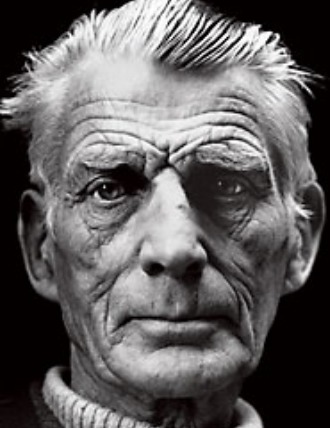
\includegraphics[width=4cm,height=4.8cm]{collection_ps/images/smith/samuel_beckett}                    \hspace{0.3cm}
    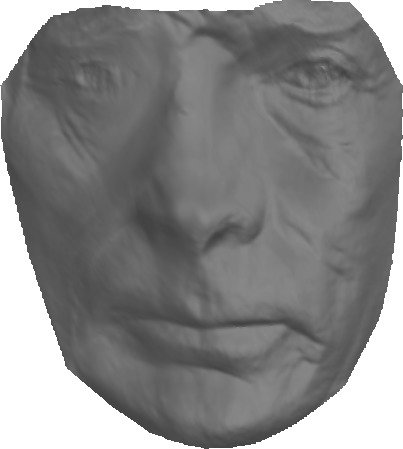
\includegraphics[width=4cm,height=4.8cm]{collection_ps/images/smith/beckett_smith_frontal_ict}         \hspace{0.3cm}
    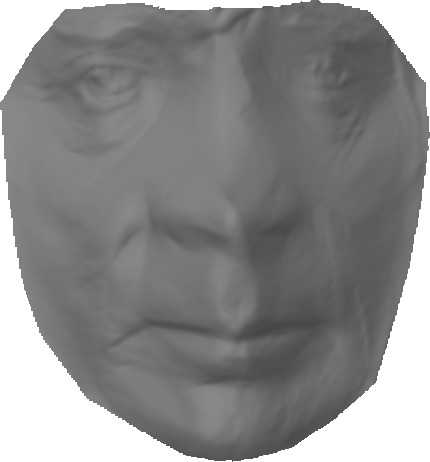
\includegraphics[width=4cm,height=4.8cm]{collection_ps/images/smith/beckett_smith_frontal_low_rank}    \\
    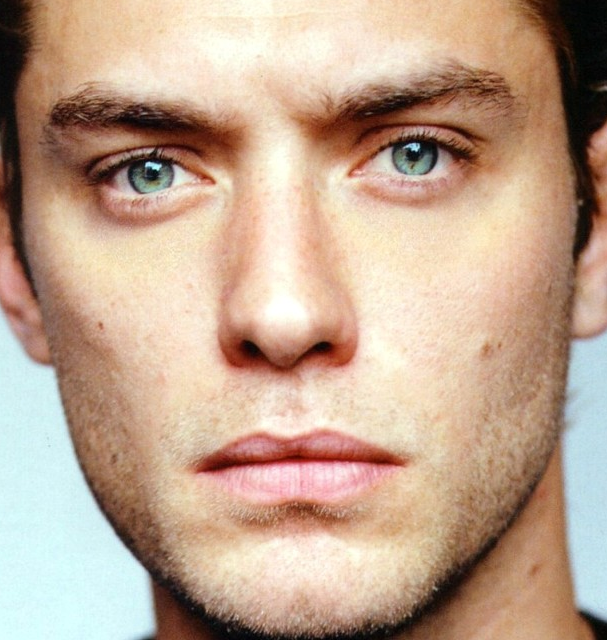
\includegraphics[width=4cm,height=4.8cm]{collection_ps/images/smith/jude_law}                          \hspace{0.3cm}
    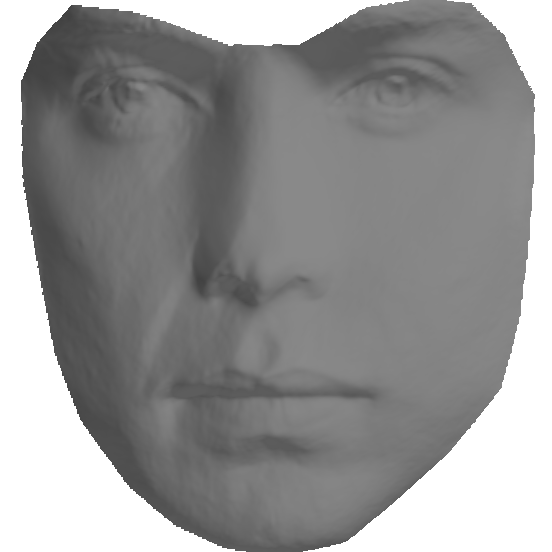
\includegraphics[width=4cm,height=4.8cm]{collection_ps/images/smith/law_smith_frontal_ict}             \hspace{0.3cm}
    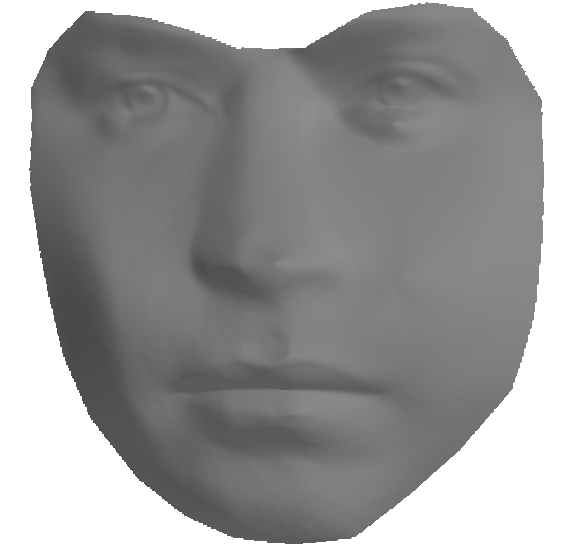
\includegraphics[width=4cm,height=4.8cm]{collection_ps/images/smith/law_smith_frontal_low_rank}
    \caption{{\bf Our subspace used for SFS}. Normals learnt automatically from 
             the Spherical Harmonic subspace of HELEN~\cite{le2012interactive} vs
             normals from the clean data of ICT-3DRFE~\cite{stratou2012exploring}.
             Middle column: the clean data. 
             Right column: proposed subspace.}
\label{fig:imag_coll_smith}
\end{figure}
%%%%%%%%%%%%%%%%%%%%%%%%%%%%%%%%%%%%%%%
The SFS technique of \citet{smith2006recovering} relies on a PCA basis
constructed from normals of a single class of object. It then seeks to recover
the high frequency normal information directly from the texture. In order to
create the PCA required by~\cite{smith2006recovering}, we recovered spherical harmonics
for every image in the dataset using the proposed algorithm. We then computed
Kernel-PCA~\cite{Snape:2014de} on the normals recovered from the HELEN images
and supplied them to~\cite{smith2006recovering}. The lighting vector is also an input to
the algorithm and we recover it by solving a least squares problem with the
known mean normals.

In order to provide a comparison for our reconstruction, we created a clean
normal subspace using the data from the ICT-3DRFE~\cite{stratou2012exploring}
database. This database is primarily use for image relighting purposes, however,
they provide a very accurate set of normals of faces under a wide range of
expressions. The results of this experiment are shown in \cref{fig:imag_coll_smith}.
Although our subspace did not provide reconstructions that are as visually
accurate as the subspace from ICT-3DRFE, they were still able to successfully
recover a plausible representation of the high frequency shading information.
%%%%%%%%%%%%%%%%%%%%%%%%%%%%%%%%%%%%%%%%%%%%%%%%%%%%%%%%%%%%%%%%
\subsection{Automatic Alignment}\label{subsec:experiments_alignment}
%%%%%%%%%%%%%%%%%%%%%%%%%%%%%%%%%%%%%%%%%%%%%%%%%%%%%%%%%%%%%%%%
%%%%%%%%%%%%%%%%%%%%%%%%%%%%%%%%%%%%%%%
\newcommand{\tomhanksalignment}[1]
{
\includegraphics[width=4cm]{collection_ps/images/tom_hanks/tom_hanks_improve_#1_initial} &
\includegraphics[width=4cm]{collection_ps/images/tom_hanks/tom_hanks_improve_#1_final}   & \hspace{0.3cm}
\includegraphics[width=4cm,height=3.8cm]{collection_ps/images/tom_hanks/tom_hanks_improve_#1_depth}
}
%%%%%%%%%%%%%%%%%%%%%%%%%%%%%%%%%%%%%%%
%%%%%%%%%%%%%%%%%%%%%%%%%%%%%%%%%%%%%%%
\setlength{\tabcolsep}{1pt}
\begin{figure}
    \centering
    \begin{tabular}{ccc}
        Initial & Final & \hspace{0.3cm} Recovered Depth \\
        \tomhanksalignment{1}                            \\
        \tomhanksalignment{129}
    \end{tabular}
    \caption{{\bf Person specific model fitting for Tom Hanks}. Images of Tom 
             Hanks coarsely aligned by a facial alignment method. Our algorithm 
             improves the facial alignment and simultaneously recovers depth. 
             Images shown are from a YouTube video of Tom Hanks.}
\label{fig:imag_coll_improve_tom_hanks}
\end{figure}
\setlength{\tabcolsep}{6pt}
%%%%%%%%%%%%%%%%%%%%%%%%%%%%%%%%%%%%%%%
%%%%%%%%%%%%%%%%%%%%%%%%%%%%%%%%%%%%%
\begin{figure}
    \hspace*{\fill}
    \begin{subfigure}[b]{0.45\textwidth}
        \centering
        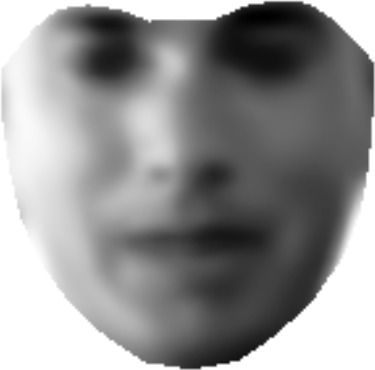
\includegraphics[width=4cm]{collection_ps/images/tom_hanks/tom_hanks_improve_0_initial}
        \caption{Start of First Iteration.}
    \end{subfigure} \hfill
    \begin{subfigure}[b]{0.45\textwidth}
        \centering
        
\includegraphics[width=4cm]{collection_ps/images/tom_hanks/tom_hanks_improve_10_final}
        \caption{End of Final (10th) Iteration.}
    \end{subfigure}
    \hspace*{\fill}
    \caption{{\bf Fitting Improvement of Tom Hanks Youtube Video}. 
             Mean of all warped frames of the Youtube video of the first and
             final iterations.}
\label{fig:imag_coll_mean_improve_tom_hanks}
\end{figure}
%%%%%%%%%%%%%%%%%%%%%%%%%%%%%%%%%%%%%
%%%%%%%%%%%%%%%%%%%%%%%%%%%%%%%%%%%%%
\newcommand{\tomhanks}[1]
{
\includegraphics[width=2.7cm,height=3.2cm]{collection_ps/images/tom_hanks/tom_hanks_#1}                   &
\includegraphics[width=2.7cm,height=3.2cm]{collection_ps/images/tom_hanks/tom_hanks_#1_low_rank}          & 
\includegraphics[width=2.7cm,height=3.2cm]{collection_ps/images/tom_hanks/tom_hanks_#1_low_rank_textured}
}
%%%%%%%%%%%%%%%%%%%%%%%%%%%%%%%%%%%%%
%%%%%%%%%%%%%%%%%%%%%%%%%%%%%%%%%%%%%
\setlength{\tabcolsep}{1pt}
\begin{figure}
    \centering
    \begin{tabular}{cccccc}
        Input & Shape & Textured & Input & Shape & Textured \vspace*{0.2cm} \\ 
        \tomhanks{14}            & \tomhanks{27}                            \\
        \tomhanks{95}            & \tomhanks{52}
    \end{tabular}
    \caption{{\bf Example reconstructions of Tom Hanks}. Images automatically 
             downloaded from Google Images. First column is the input images, 
             second column is the untextured shape from the proposed technique 
             and the third column is the textured shape.}
\label{fig:imag_coll_tom_hanks}
\end{figure}
\setlength{\tabcolsep}{6pt}
%%%%%%%%%%%%%%%%%%%%%%%%%%%%%%%%%%%%%
In this experiment we used the Active Template Model (ATM) provided by the Menpo
project~\cite{menpo14} in order to perform a project-out type algorithm to align
images of Tom Hanks. This model is similar to the Lucas-Kanade
\cite{lucas1981iterative} method but uses a point distribution model (PDM) in order to
perform non-rigid alignment between the images. In particular, the template
image is fixed during optimisation of the PDM, and we use our subspace to
provide a texture representing an approximation of the diffuse component of the
image. This is essentially identical to the procedure performed within a
project-out AAM.\@

We used a person specific SH subspace that was built on images of Tom Hanks that
were downloaded automatically from the Internet. In this case, the images were
automatically aligned using the DLib implementation of~\cite{kazemi2014one}. For
this experiment, $k = 30$ and thus the total number of components $4k = 120$. We
downloaded 200 frames from a Youtube video of Tom
Hanks\footnote{\url{https://www.youtube.com/watch?v=nFvASiMTDz0} from 3:43} and
attempted to automatically align them using our subspace and the ATM.\@ The ATM
was initialised using another fitting of~\cite{kazemi2014one} which was then
iteratively improved. At each global iteration, we recovered a new set of
diffuse textures for each frame and then performed a refitting of every frame.
This caused the images to align over a sequence of iterations. We performed 10
such iterations. \cref{fig:imag_coll_improve_tom_hanks} shows two example frames
where the alignment was improved and dense shape was also recovered.
%%%%%%%%%%%%%%%%%%%%%%%%%%%%%%%%%%%%%%%%
\newcommand{\yaleb}[1]
{
\includegraphics[width=4cm,height=4.5cm]{collection_ps/images/yaleb_results/yale_b_#1}                      & \hspace{1.5cm} 
\includegraphics[width=4cm,height=4.5cm]{collection_ps/images/yaleb_results/yale_b_#1_photometric}          & \hspace{1.5cm}
\includegraphics[width=4cm,height=4.5cm]{collection_ps/images/yaleb_results/yale_b_#1_photometric_low_rank}
}
\setlength{\tabcolsep}{1pt}
\begin{figure}
    \centering
    \begin{tabular}{ccc}
        Input & \hspace{1.5cm} Photometric Stereo & \hspace{1.5cm} Proposed  \vspace*{0.2cm} \\ 
        \yaleb{B01}                            \\
        \yaleb{B03}                            \\
        \yaleb{B06}                                                  
    \end{tabular}
    \caption{{Examples comparing against traditional Photometric Stereo}. 
             Images from the Yale B dataset~\cite{georghiades2001fromfew}. 
             First column is the input images, second column is traditional 
             PS result and the third column is the proposed algorithm.}
\label{fig:imag_coll_yale_b}
\end{figure}
\setlength{\tabcolsep}{6pt}
%%%%%%%%%%%%%%%%%%%%%%%%%%%%%%%%%%%%%%%%
%%%%%%%%%%%%%%%%%%%%%%%%%%%%%%%%%%%%%%%%
\newcommand{\comparemm}[1]
{
\includegraphics[width=3cm,height=3.5cm]{collection_ps/images/helen/helen_#1}                 & \hspace{0.2cm}
\includegraphics[width=3cm,height=3.5cm]{collection_ps/images/helen/helen_#1_frontal_vizago}  & \hspace{0.2cm}
\includegraphics[width=3cm,height=3.5cm]{collection_ps/images/helen/helen_#1_side_vizago}     & \hspace{0.2cm}
\includegraphics[width=3cm,height=3.5cm]{collection_ps/images/helen/helen_#1_frontal_facegen} & \hspace{0.2cm}
\includegraphics[width=3cm,height=3.5cm]{collection_ps/images/helen/helen_#1_side_facegen}
}
\setlength{\tabcolsep}{1pt}
\begin{figure*}
    \centering
    \begin{tabular}{ccccc} \vspace*{0.2cm}
        Input & \multicolumn{2}{c}{vizago.ch} & \multicolumn{2}{c}{facegen.com}  \\
        \comparemm{6}                                                            \\
        \comparemm{680}                                                          \\
        \comparemm{821}                  
    \end{tabular}
    \caption{{\bf Examples of difficult reconstructions for existing commercial 
              Morphable Model implementations}. 
             Images from the HELEN~\cite{le2012interactive} dataset. 
             Both implementations do not provide the ability to render 
             textureless surfaces.
             Facegen.com reported invalid landmarks for the image given in the
             first row.}
\label{fig:imag_coll_helen_compare_morphable_model}
\end{figure*}
\setlength{\tabcolsep}{6pt}
%%%%%%%%%%%%%%%%%%%%%%%%%%%%%%%%%%%%%%%%
%%%%%%%%%%%%%%%%%%%%%%%%%%%%%%%%%%%%%%%%
\newcommand{\comparehelen}[2]
{
\includegraphics[width=2.5cm,height=2.5cm]{collection_ps/images/helen/helen_#1}                  & \hspace{0.5cm}
\includegraphics[width=2.3cm,height=2.5cm]{collection_ps/images/helen/helen_#1_frontal_low_rank} & \hspace{0.5cm}
\includegraphics[width=2.3cm,height=2.5cm]{collection_ps/images/helen/helen_#1_frontal_ira}      & \hspace{0.5cm}
\includegraphics[width=3cm,height=2.5cm]{collection_ps/images/helen/helen_#1_#2_low_rank}        & \hspace{0.5cm}
\includegraphics[width=3cm,height=2.5cm]{collection_ps/images/helen/helen_#1_#2_ira}
}
\begin{landscape}
\thispagestyle{footeronly}
\setlength{\tabcolsep}{1pt}
\begin{figure*}
    \centering
    \begin{tabular}{ccccc} \vspace*{0.2cm}
        Input & \hspace{0.5cm} Proposed & \hspace{0.5cm}~\cite{KemelmacherShlizerman:2013iv} & \hspace{0.5cm} Proposed & \hspace{0.5cm}~\cite{KemelmacherShlizerman:2013iv} \\
        \vspace*{-0.1cm}
        \comparehelen{1348}{side} \\ \vspace*{-0.07cm}
        \comparehelen{555}{side}  \\ \vspace*{-0.07cm}
        \comparehelen{680}{chin}  \\ \vspace*{-0.07cm}
        \comparehelen{6}{chin}    \\ \vspace*{-0.07cm}
        \comparehelen{821}{side}  \\ \vspace*{-0.07cm}
        \comparehelen{77}{side}                                      
    \end{tabular}
    \caption{{\bf Comparison with the least-squares decomposition 
             of~\cite{KemelmacherShlizerman:2013iv}}.
             Images from the HELEN~\cite{le2012interactive} dataset.}
\label{fig:imag_coll_helen_compare}
\end{figure*}
\setlength{\tabcolsep}{6pt}
\end{landscape}
%%%%%%%%%%%%%%%%%%%%%%%%%%%%%%%%%%%%%%%%

%%%%%%%%%%%%%%%%%%%%%%%%%%%%%%%%%%%%%%%%%%%%%%%%%%%%%%%%%%%%%%%%%%%%%%%%%%%%%%%%
\section{Summary and Conclusion}\label{sec:imag_coll_summary}
%%%%%%%%%%%%%%%%%%%%%%%%%%%%%%%%%%%%%%%%%%%%%%%%%%%%%%%%%%%%%%%%%%%%%%%%%%%%%%%%
In this chapter we investigated 3D facial shape recovery on collections of
``in-the-wild'' images. This is a challenging scenario as no knowledge of the
lighting conditions, the facial location or the camera geometric properties is
provided. However, by leveraging the large number of images and the inherent
low-rank properties of the human face we have shown that plausible 3D shape
can be recovered without any 3D prior. We have provided an optimisation
framework for the recovery and separation of both the illumination and
deformation parameters of a spherical harmonic subspace. Most importantly,
this optimisation framework contains low-rank constraints that mitigate the
effect of common sparse image outliers such as occlusions. We also demonstrated
that a global and sparse alignment is sufficient for recovering plausible shape
without the need for expensive per pixel alignment such as optical flow.

We have evaluated our algorithm qualitatively on it's ability to recover
plausible facial shape on the ``in-the-wild'' HELEN~\cite{le2012interactive}
and demonstrate robustness to occlusions. This is particularly evident when
qualitatively compared to the least-squares solution as originally proposed by
\citet{KemelmacherShlizerman:2013iv}. We have also shown that our algorithm,
due to the single global template space, is applicable for 
GSFS (\cref{sec:singl_img_gsfs}) and iterative person specific image alignment
and depth recovery. Unfortunately, there lacks a standard benchmark for
3D surface recover from images using image formation techniques. Thus we provide
relatively few quantitative experiments and rely on the perception of our
recovered shape as is common in other works in the
area~\cite{KemelmacherShlizerman:2013iv,kemelmacher2011face,kemelmacher2012collection}.

Although the recovery of plausible normals directly from images, without any
3D prior, is an attractive problem, it still does not recover shapes that
are visually comparable to techniques that employ an explicit 3D prior. Therefore,
in the next chapter we investigate another form of the image collection problem,
where temporal consistency is assumed. We formulate the problem as one of alignment
and use an explicit 3D model in order to recover 3D shape implicitly as part
of the alignment output.

%%%%%%%%%%%%%%%%%%%%%%%%%%%%%%%%%%%%%%%%%%%%%%%%%%%%%%%%%%%%%%%%%%%%%%%%%%%%%%%%
\stopcontents[chapters]
%%%%%%%%%%%%%%%%%%%%%%%%%%%%%%%%%%%%%%%%%%%%%%%%%%%%%%%%%%%%%%%%%%%%%%%%%%%%%%%%
